\documentclass{lhcbnote}
\usepackage{longtable}
\usepackage{rotating}
\usepackage{tikz}
\usetikzlibrary{shapes,arrows}
\usepackage[active,tightpage]{preview}
\PreviewEnvironment{tikzpicture}

\title{SALT128 Wafer Screening}
%\author{Benjamin Gaidioz{\address[BGADD]{CERN,Switzerland}},}
%for more than one author 
\author{Christopher Betancourt, Iaroslava Bezshyiko {\address{University of Zurich, Switzerland}}
%with a different address
%}
}

\doctyp{Internal Note}
\dociss{1}
\docrev{0}
\docref{LHCb-XX-2017}
\doccre{February 8, 2017}
\docmod{\today}
%\doccnf{You use this command only if you want a note 
%here: like presented at...}

\begin{document}

\maketitle

\begin{abstract}
This is a description of wafer probe tests for the SALT128 mass production quality assurance. The mechanical and electrical layout of the chip as relevant for the tests, types of tests to be carried out, information on the wafer probe card and a timeline is provided.
\end{abstract}

%\begin{status}
%\entry{Draft}{1}{December 3, 2003}{First version. Introduction only,
%conclusion is missing}
%\entry{Draft}{2}{December 16, 2003}{Added conclusion.}
%\entry{Final}{1}{April 26, 2004}{Checked english}
%\end{status}

\tableofcontents

\listoffigures
\listoftables

\section{Introduction}
SALT (\textbf{S}ilicon \textbf{A}SIC for \textbf{L}HCb \textbf{T}racking) is a 128 channel ASIC to be used as a readout chip for silicon sensors in the UT of LHCb experiment. Quality assurance tests need to be carried out after mass production of the chip, insuring high yield and proper functionality before installation into the experiment. The large volume of chips ($\sim$ 5k) requires tests to be carried out in an automatic fashion, with each chip classified into three catagories; GOOD (full functionality of every channel), OK (at most one bad channel) and BAD (two or more bad channels). The chips will be tested on wafer before dicing.

Tests will be carried out with a semi-automatic probe station housed in a clean room located at CERN. The probe station is equipped with special imaging allowing for proper alignment and planarity. A wafer probe card will be used to make electrical contact with the chip. The probe card will be connected to a DAQ system controlled by a PC which also controls power supplies and movement of the probe station chuck, as illustrated in figure \ref{fig:test_sum}.

\begin{figure}
\centering
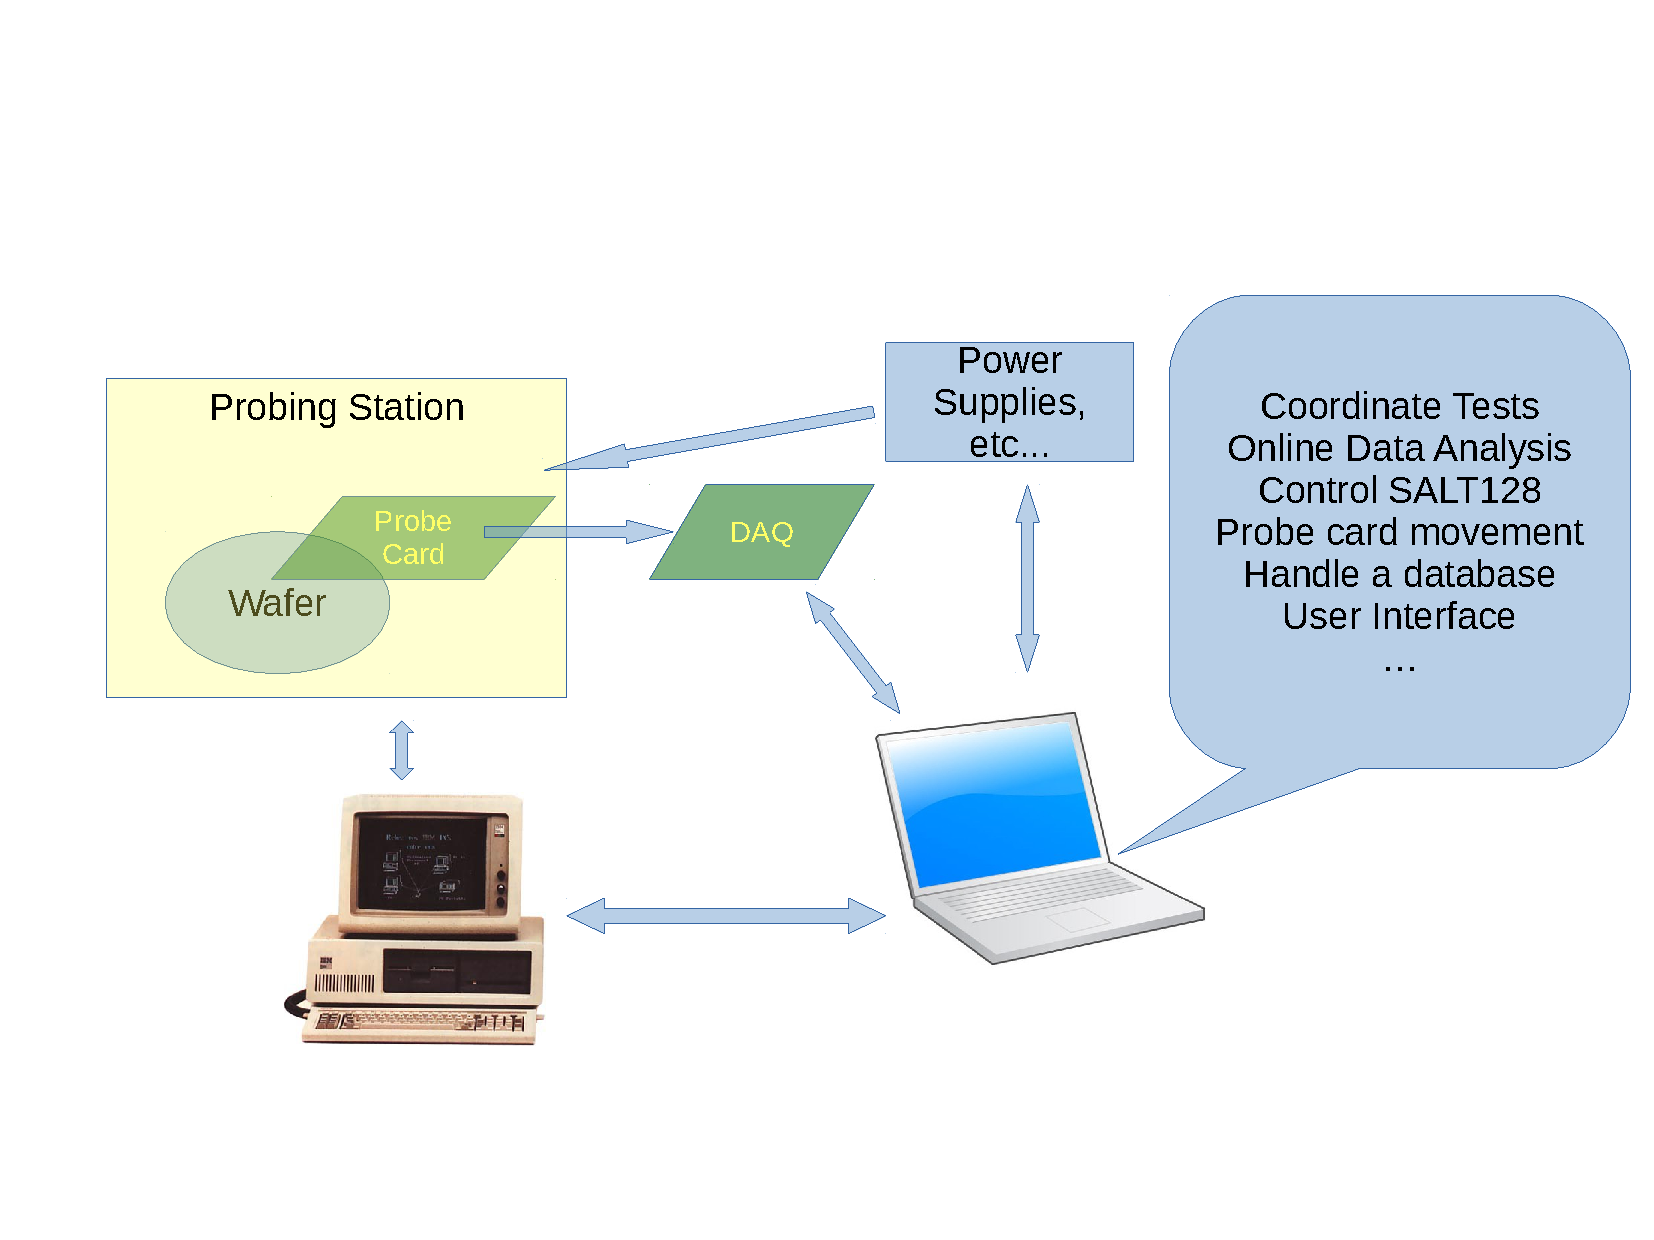
\includegraphics[width=\textwidth]{figures/test_sum}
\caption{Illustration of the measurement set up.}
\label{fig:test_sum}
\end{figure}

%%%%%%%%%%%%%%%%%%%%%%%%%%%%%%%%%%%%%%%%%%%%%%%%%%

\section{SALT128 layout}

SALT128 will contain a total of 246 pads: 128 input pads which will not be probed during the wafer probe tests and will be bonded to hybrids after screening, 4 ground pads, two on each side of the 128 input pads, 78 pads on the opposite to the input pads which will be tested during wafer screening and also subsequently bonded to hybrid, and two sets of 18 pads which will only be used during wafer screening. A layout of the chip indicating the pad locations and their pin numbers is shown in figure \ref{fig:pads}. A list of pads to be probed during wafer screening is indicated in table \ref{table:pin}.

\begin{figure}
\centering
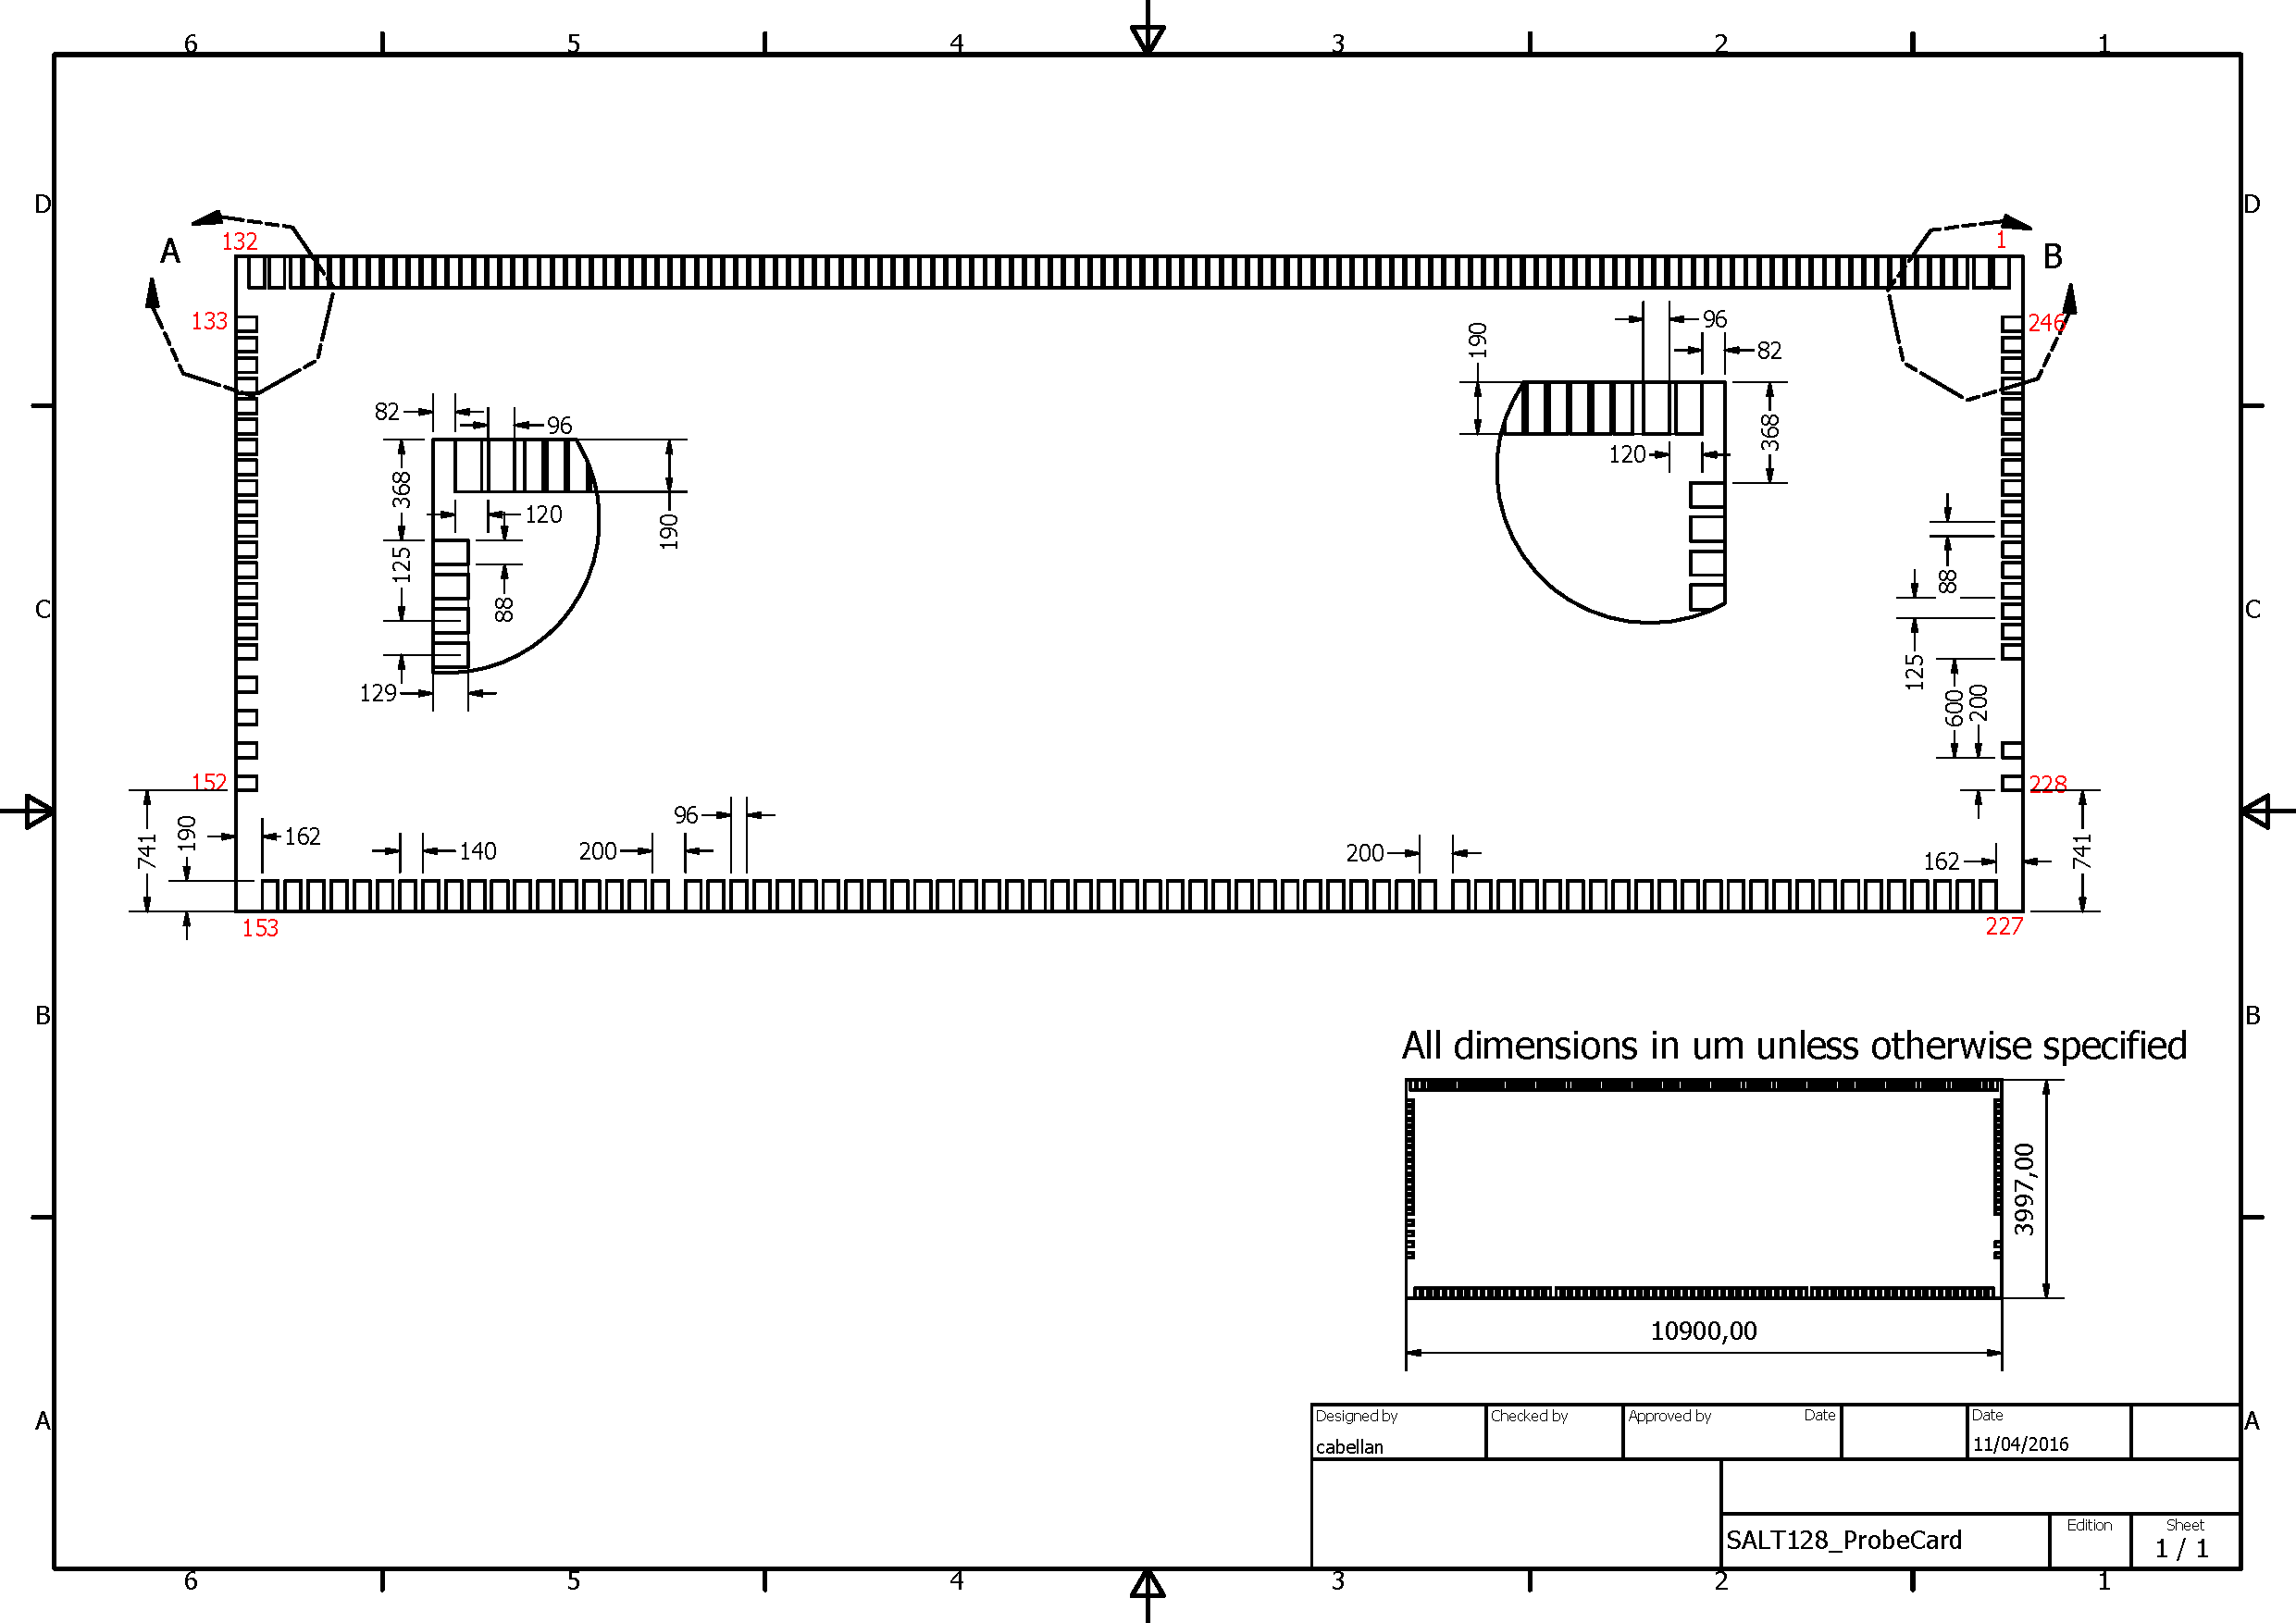
\includegraphics[width=\textwidth]{figures/SALT128_ProbeCard}
\caption{Layout of the pads on SALT128.}
\label{fig:pads}
\end{figure}

%\begin{longtable}
%\resizebox{\textwidth}{!}{
\begin{longtable}{ | l | l | l | }
%\centering
\hline
	Pin & Name & Probed? \\ \hline
	1 & VSSAI & ? \\ \hline
	2 & VSSAI & ? \\ \hline
	131 & VSSAI & ? \\ \hline
	132 & VSSAI & ? \\ \hline
	133 & PRE\_BUF1 & weak no \\ \hline
	134 & SH1\_BUF1 & weak no \\ \hline
	135 & SH2\_BUF1 & weak no \\ \hline
	136 & SH\_BUF1 & weak no \\ \hline
	137 & AP\_BUF1 & weak no \\ \hline
	138 & AN\_BUF1 & weak no \\ \hline
	139 & I\_BUF1 & weak no \\ \hline
	140 & VSSPSTD\_BUF1 & weak no \\ \hline
	141 & VSSA\_BUF1 & YES \\ \hline
	142 & VDDA\_BUF1 & YES \\ \hline
	143 & ADC\_INP & weak no \\ \hline
	144 & ADC\_INN & weak no \\ \hline
	145 & V\_S2D\_DAC & YES \\ \hline
	146 & V\_PULSE\_DAC & YES \\ \hline
	147 & V\_SLVS\_VBIAS\_DAC & YES \\ \hline
	148 & V\_SLVS\_INREF\_DAC & YES \\ \hline
	149 & SCAN\_ENABLE & YES \\ \hline
	150 & SDI & YES \\ \hline
	151 & SDO & weak no \\ \hline
	152 & TEST\_MODE & YES \\ \hline
	153 & VDD & YES \\ \hline
	154 & VSS & YES \\ \hline
	155 & VDD & YES \\ \hline
	156 & VSS & YES \\ \hline
	157 & VDDPST & YES \\ \hline
	158 & ID0 & YES \\ \hline
	159 & ID1 & YES \\ \hline
	160 & ID2 & YES \\ \hline
	161 & I2C\_SCL & YES \\ \hline
	162 & I2C\_SDA & YES \\ \hline
	163 & RST\_N & YES \\ \hline
	164 & MAIN\_CLK\_N & YES \\ \hline
	165 & MAIN\_CLK\_P & YES \\ \hline
	166 & VSSPST & YES \\ \hline
	167 & VDD & YES \\ \hline
	168 & VSS & YES \\ \hline
	169 & VDD & YES \\ \hline
	170 & VSS & YES \\ \hline
	171 & VDDAPST & YES \\ \hline
	172 & VSSAPST & YES \\ \hline
	173 & VDDADC & YES \\ \hline
	174 & VSSADC & YES \\ \hline
	175 & VDDADC & YES \\ \hline
	176 & VSSADC & YES \\ \hline
	177 & VREFD & YES \\ \hline
	178 & VSSADC & YES \\ \hline
	179 & VREFD & YES \\ \hline
	180 & VSSADC & YES \\ \hline
	181 & VDDADC & YES \\ \hline
	182 & VSSADC & YES \\ \hline
	183 & VDDADC & YES \\ \hline
	184 & VSSVCM & YES \\ \hline
	185 & VDDVCM & YES \\ \hline
	186 & VSSVCM & YES \\ \hline
	187 & VDDVCM & YES \\ \hline
	188 & VSSAPST\_IN & YES \\ \hline
	189 & VDDAPST\_IN & YES \\ \hline
	190 & VSSAPST\_IN & YES \\ \hline
	191 & VDDAPST\_IN & YES \\ \hline
	192 & VSSAI & YES \\ \hline
	193 & VDDA & YES \\ \hline
	194 & VSSAI & YES \\ \hline
	195 & VDDA & YES \\ \hline
	196 & VSSAI & YES \\ \hline
	197 & VDDA & YES \\ \hline
	198 & VSSA & YES \\ \hline
	199 & VDDA & YES \\ \hline
	200 & VSSA & YES \\ \hline
	201 & VDDA & YES \\ \hline
	202 & VSSA & YES \\ \hline
	203 & VDDA & YES \\ \hline
	204 & VSS & YES \\ \hline
	205 & VDD & YES \\ \hline
	206 & VSS & YES \\ \hline
	207 & VDD & YES \\ \hline
	208 & VSSPST & YES \\ \hline
	209 & DDR\_TFC\_N & YES \\ \hline
	210 & DDR\_TFC\_P & YES \\ \hline
	211 & DDR\_OUT0\_N & YES \\ \hline
	212 & DDR\_OUT0\_P & YES \\ \hline
	213 & DDR\_OUT1\_N & YES \\ \hline
	214 & DDR\_OUT1\_P & YES \\ \hline
	215 & DDR\_OUT2\_N & YES \\ \hline
	216 & DDR\_OUT2\_P & YES \\ \hline
	217 & DDR\_OUT3\_N & YES \\ \hline
	218 & DDR\_OUT3\_P & YES \\ \hline
	219 & DDR\_OUT4\_N & YES \\ \hline
	220 & DDR\_OUT4\_P & YES \\ \hline
	221 & DDR\_OUT5\_N & YES \\ \hline
	222 & DDR\_OUT5\_P & YES \\ \hline
	223 & VDDPST & YES \\ \hline
	224 & VSS & YES \\ \hline
	225 & VDD & YES \\ \hline
	226 & VSS & YES \\ \hline
	227 & VDD & YES \\ \hline
	228 & DATA\_CLK\_OUT\_N & YES \\ \hline
	229 & DATA\_CLK\_OUT\_P & YES \\ \hline
	230 & V\_SH\_DAC & YES \\ \hline
	231 & V\_KRUM\_DAC & YES \\ \hline
	232 & V\_PRE\_DAC & YES \\ \hline
	233 & VMCD & YES \\ \hline
	234 & VCMC & YES \\ \hline
	235 & VCMB & YES \\ \hline
	236 & VCMA & YES \\ \hline
	237 & VDDA\_BUF0 & weak no \\ \hline
	238 & VSSA\_BUF0 & weak no \\ \hline
	239 & VSSPSTD\_BUF0 & weak no \\ \hline
	240 & I\_BUF0 & weak no \\ \hline
	241 & AN\_BUF0 & weak no \\ \hline
	242 & AP\_BUF0 & weak no \\ \hline
	243 & SH\_BUF0 & weak no \\ \hline
	244 & SH2\_BUF0 & weak no \\ \hline
	245 & SH1\_BUF0 & weak no \\ \hline
	246 & PRE\_BUF0 & weak no \\ \hline
%\end{tabular}
\caption{List of pads to be tested during wafer screening.}
\label{table:pin}
%}
\end{longtable}



\section{Probe station, wafer probe card and DAQ}

All wafer probe tests will make use of a semi-automatic probe station located in a clean room at CERN. A photo of the set up is shown in figure \ref{fig:probe_station}. 

\begin{sidewaysfigure}
\centering
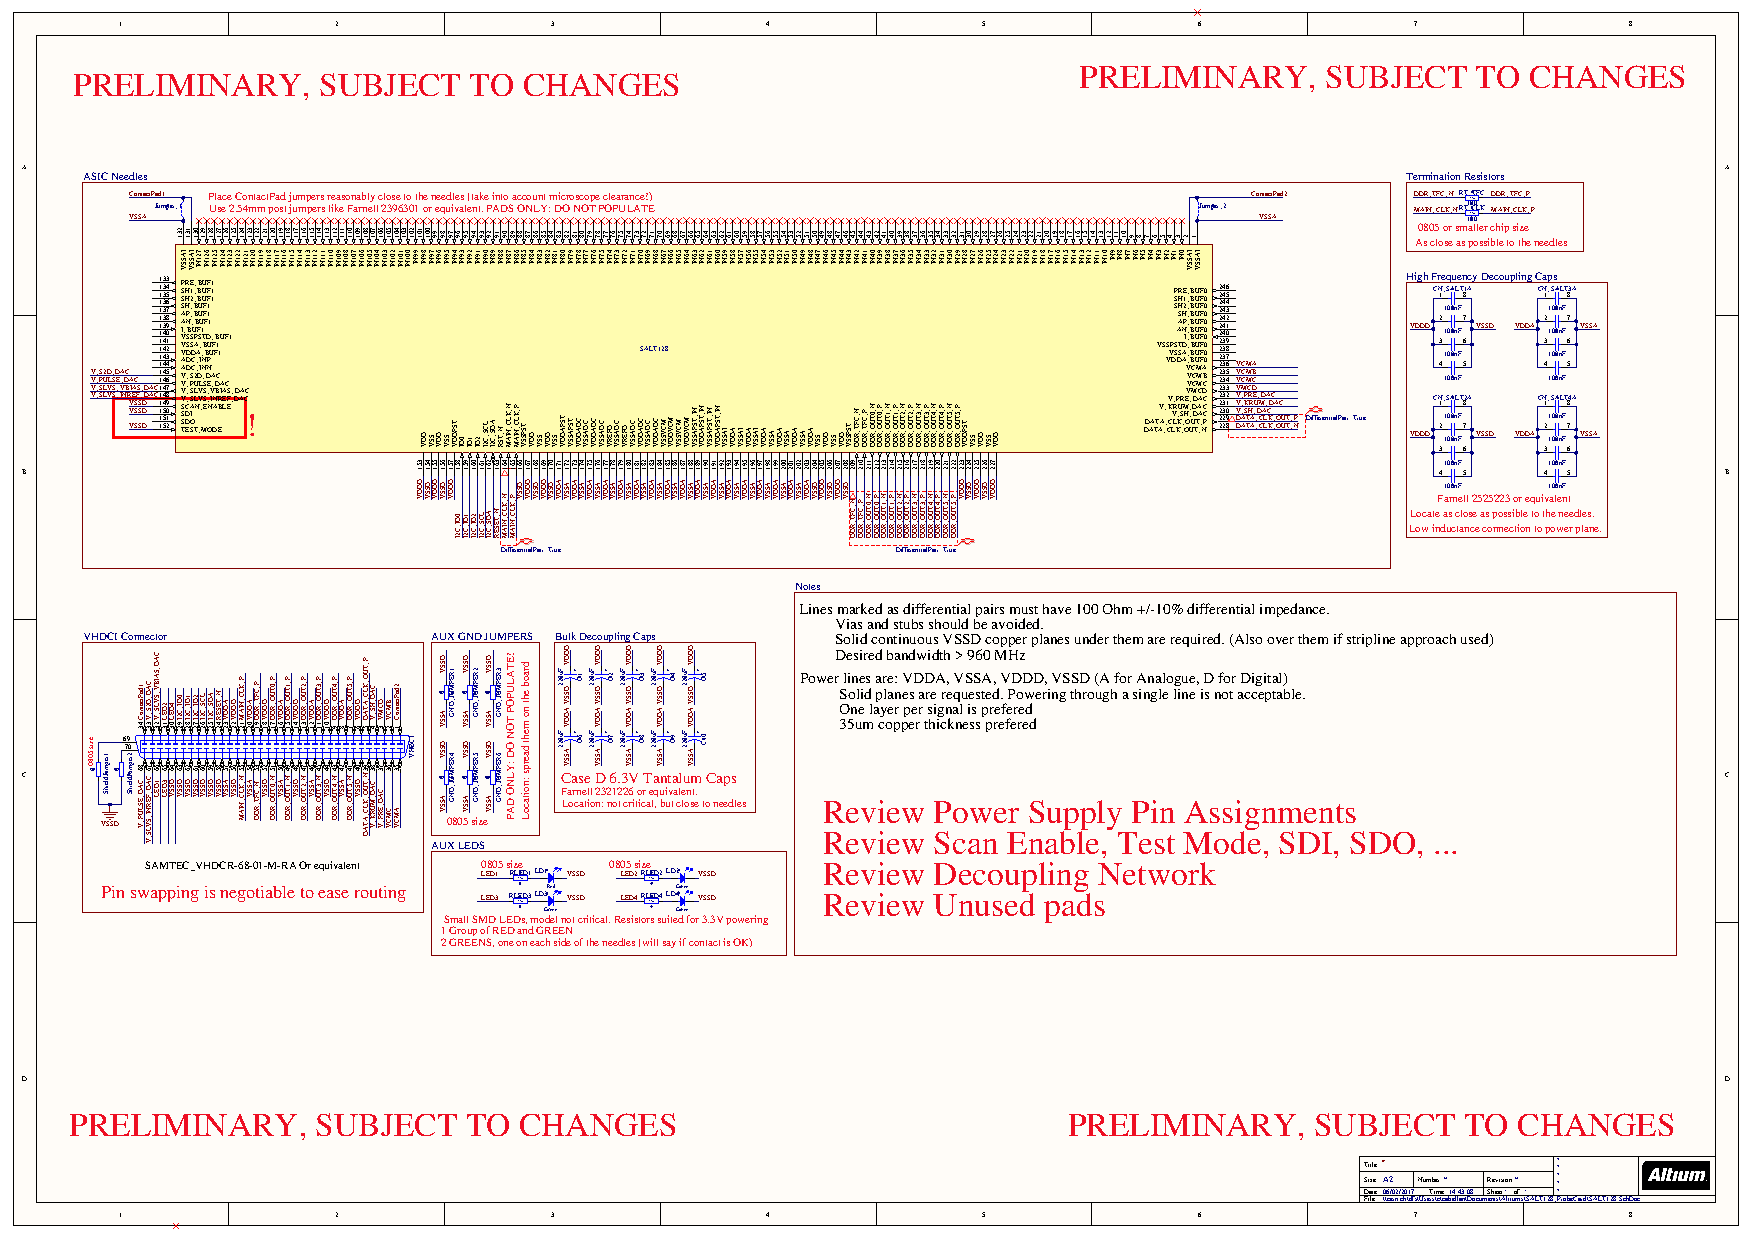
\includegraphics[width=\textwidth]{figures/SALT128}
\caption{Schematic of the SALT128 chip with the input pads labeled and lines to the DAQ.}
\label{fig:salt}
\end{sidewaysfigure}

\begin{figure}
\centering
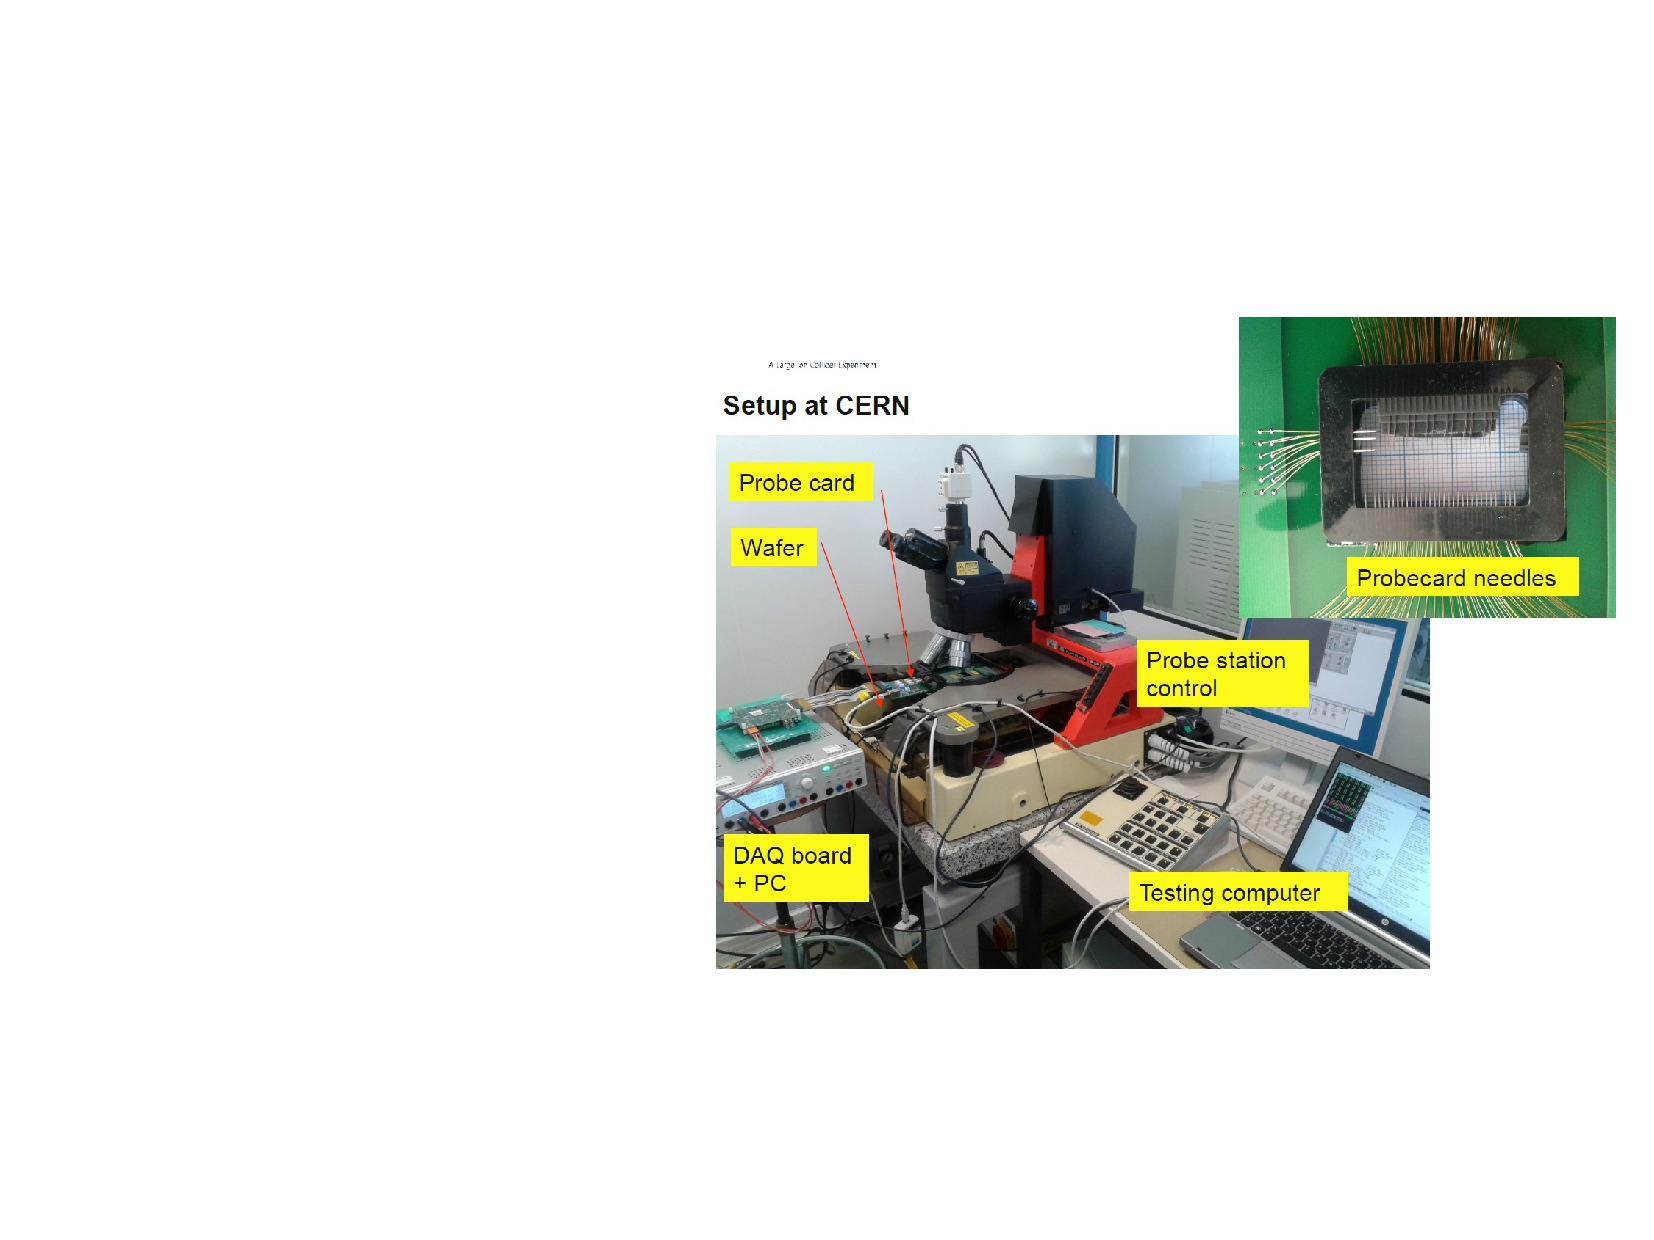
\includegraphics[width=\textwidth]{figures/probe_station}
\caption{Picture of the semi-automatic probe station with connections to the PCs and DAQ (PRILIMARY PICTURE, TAKEN FROM \textit{P. Riedler, 5th ALICE ITS, MFT and O2 Meeting}).}
\label{fig:probe_station}
\end{figure}

%%%%%%%%%%%%%%%%%%%%%%%%%%%%%%%%%%%%%%%%%%%%%%%%%%

\section{Functionality}

The SALT ASIC, containing 128 channels and an additional two channels for testing and monitoring, is broken into several components:
\begin{itemize}
\item \textbf{Analogue front-end} - Each channel on the front-end consists of a preamplifier, a shaper and a signal-to-differential converter.
\item \textbf{Analog to Digital Converter} - Each channel contains a 6-bit ADC. An additional six ADCs a present for monitoring.
\item \textbf{DACs} - Seven DACs used to bias different blocks of the SALT chip. Additionally, each channel contains a 7-bit DAC to set the front-end baseline voltage.
\item \textbf{Clock generation} - 40 MHz external clock is used in the digital part of the chip. A DLL is used to shift this clock to get the ADC signal and generate test pulses. An internal PLL is used to obtain a fast 160 MHz clock for sterilization and transmission of data.
\item \textbf{Digital Signal Processing} - Signal processing performs pedestal subtraction, mean CMS, and zero suppression.
\item \textbf{Back-end processing} - Processing after the DSP chain is associated with the TFC commands.
\end{itemize}

%%%%%%%%%%%%%%% TYPE OF TESTS SECTION %%%%%%%%%%%%%%%
\section{Tests to be performed}

\begin{itemize}
\item \textbf{Power tests} - Need to test proper start up of the chip. Make sure the digital and analogue currents are being drawn correctly. Need to simulate working conditions for the LHCb UT by applying expected trigger rate.
\item \textbf{DAC tests} - Record output of each DAC over range of possible values to confirm proper behavior.
\item \textbf{Digital tests} - Make sure the chip can be configured. This includes being able to read/write registers, read chip addresses, pass signals in both directions.
\item \textbf{Analogue tests} - Should perform five point gain tests (inject five different charges) and read out ADC values to assess analogue functionality.
\item \textbf{Gain uniformity} - Check output signal uniformity across channels for a given input. Should test for different input charge.
\item \textbf{Clock checks} - Check different phase shifts of the clock and data lines to confirm optimal value.
\item \textbf{Cross-talk studies} - Confirm that cross-talk is less than 5\% between neighboring channels.
\item \textbf{Pedestal and CMS} - Check proper Pedestal subtraction and CMS.
\item \textbf{Noise studies} - Measure the intrinsic and CMS noise per channel.
\end{itemize}

%%%%%%%%%%%%%%% MEASUREMENT DETAILS SECTION %%%%%%%%%%%%%%%
\section{Measurement details}

\subsection{Power tests}

Perhaps the single most important test is that of power consumption. In the majority of cases, if the chip draws the correct current, then most of the functionality should work properly. On the other had, a large deviation from the expected power consumption usually indicates a serious issue or defective chip. These tests will be performed using external ADCs.

Two power consumption tests per chip are envisioned:

\begin{itemize}
\item Power consumption test right after powering up SALT128.
\item Power consumption test after all other tests once the chip has been fully configured.
\end{itemize}
Both tests should check if the current being drawn is within $\pm 20 \%$ of expectations, otherwise the chip is flagged as BAD.

\subsection{Digital communication}
SALT communicates with the outside world with three interfaces: a slow (100 KHz) I$^2$C read-write interface that controls all digital logic of the chip; two fast (320 Mb/s) read (TFC) and write (DAQ) interfaces. Proper chip functionality requires testing of all three interfaces as well as proper clock configuration and synchronization (DLL and PLL).

\begin{itemize}
\item \textbf{I$^2$C} - Testing proper I$^2$C involves ensuring proper writing and reading of registers. This is accomplished with the \texttt{pattern\_cfg} register of the Serializer. 1/10$^6$ incorrect bits indicates a faulty chip, thus about 200k patterns need to be tested. \\
Test details
\begin{enumerate}
\item Reset and make sure I$^2$C is not busy.
\item Configure PLL by writing b10001101 to the \texttt{pll\_main\_cfg} register. If unable to configure, flag chip as BAD. 
\item Write a random bit pattern to the \texttt{pattern\_cfg} register. Read back the pattern in the \texttt{pattern\_cfg} register and make sure it is the same as was written. If the read pattern is different than the written one, then flag the chip as BAD.
\item Reapeat step 3. 200k times.
\end{enumerate}
\item \textbf{DLL configuration} - The following configuration of the DLL is based on section 5.1.1 of the SALT ver 3 chip documentation. \\
Test details
\begin{enumerate}
\item Set correct value of CP current by writing \texttt{h9A} to the \texttt{dll\_cp\_cfg} register.
\item Set start value of \texttt{h60} to the \texttt{dll\_vcdl\_cfg} register.
\item Wait for 1 $\mu$s.
\item Read \texttt{dll\_cur\_ok} bit from the \texttt{dll\_vcdl\_mon} register and make sure it is 0, otherwise increase start value of \texttt{dll\_vcdl\_cfg} by 1.
\item Repeat step 4 until \texttt{dll\_cur\_ok} bit from the \texttt{dll\_vcdl\_mon} register is 0. If failure to reach 0 after N tries, then classify chip as BAD.
\item Decrease \texttt{dll\_vcdl\_cfg} by 1.
\item Wait for 1 $\mu$s.
\item Read \texttt{dll\_cur\_ok} bit from the \texttt{dll\_vcdl\_mon} register and make sure it is 0, otherwise decrease start value of \texttt{dll\_vcdl\_cfg} by 1.
\item Repeat step 8 until \texttt{dll\_cur\_ok} bit from the \texttt{dll\_vcdl\_mon} register is 0. If failure to reach 0 after N tries, then classify chip as BAD.
\item Set \texttt{dll\_start} to 1
\item Read the \texttt{dll\_vcdl\_voltage} bits in the \texttt{dll\_vcdl\_mon} register and make sure this is 0. A value of $\pm 8$ is also acceptable, although suboptimal. If value is outside this range, then flag chip as BAD.
\end{enumerate}
\item \textbf{PLL configuration} - The following configuration of the PLL is based on section 5.2.1 of the SALT ver 3 chip documentation. \\
Test details
\begin{enumerate}
\item Make sure PLL is configured by reading the \texttt{pll\_main\_cfg} register and making sure it is set to  b10001101. If not, write b10001101 to the \texttt{pll\_main\_cfg} register.
\item Read value of the \texttt{pll\_cp\_cfg} register. If not the default value of b10011010, then write b10011010 to the \texttt{pll\_cp\_cfg} register.
\item Read value of the \texttt{pll\_vco\_cur} bits in the \texttt{pll\_vco\_cfg} register.
\item If value of the \texttt{pll\_vco\_cur} is equal to $0\pm8$, then PLL is properly configured.
\end{enumerate}
\item \textbf{DAQ-clock synchronization} - Checking proper functionality of the DAQ lines (E-links) requires synchronization with the clock using a known pattern and making sure pattern can be read out properly. The chosen pattern will be \texttt{hAB}.
\begin{enumerate}
\item Set the correct pattern for synching by writing \texttt{hAB} to the \texttt{pattern\_cfg} register.
\item Reset \texttt{ser\_source\_cfg} and set output of DAQ to the pattern by writing \texttt{h22} to the \texttt{ser\_source\_cfg} register.
\item Reset DAQ by writing \texttt{h01} to the \texttt{DAQ\_CFG} FPGA register.
\item Clear FPGA FIFO by writing \texttt{h10} to the \texttt{DAQ\_CFG} FPGA register.
\item Start a synchronization cycle by writing \texttt{h02} to teh \texttt{DAQ\_CFG} FPGA register.
\item Continuously read the \texttt{DAQ\_CFG} FPGA register until it b2 reads 1, which indicates that the synchronization procedure is done and all e-links have seen at least one good synchronization. 
\item Properly read the output of the E-links and make sure the correct pattern (\texttt{hAB}) is being read out. If output is \texttt{hAB}, wait 1 us and go back to step 3.
\item If synchronization fails, i.e. if read back pattern is not \texttt{hAB}, then need to shift phase in PLL. This can be done by writing \texttt{h01} to register 0x40018 (PLL register, no name yet) of the FPGA, which defines the phase to shift by 1/8 of the clock period, and writing 1 to b5 of the register 0x40020 of the FPGA, which defines the shift to increment up.
\item Make sure you can synchronize 10k times in a row. If yes, then synchronization complete, otherwise flag chip as BAD.
\end{enumerate}
\item \textbf{TFC check} - There are 8 TFC commands that are recognized by SALT as outlined in the SALT manual: BXReset, FEReset, Header, NZS, BxVeto, Snapshot, Synch, and Calib. Here we test some basic commands: BXReset, FEReset, Heaser and BxVeto, . \\
Test details
\begin{enumerate}
\item Reset the TFC state machine and set all related registers to default values. This is done by writing b0=1 in the \texttt{TFC\_CFG} FPGA register.
\item Set TFC to single transmission by writing 1 to b1 in the \texttt{TFC\_CFG} FPGA register.
\item Set the appropriate Sync data packets to their reset values by writing to the \texttt{syncX\_cfg} registers. 
\item Reset the BXID counter and define Sync data output. First define the TFC length (number of commands, in this case 2) by writing \texttt{h02} to the \texttt{TFC\_LENGTH} FPGA register. To reset the BXID, write b00000001 to the \texttt{TFC\_WR} FPGA register. Next set the Sync command by writing b01000000 to the \texttt{TFC\_WR} FPGA register. Write \texttt{h01} to the \texttt{TFC\_TRIGGER} FPGA register to begin TFC command execuation.
\item Keep reading the \texttt{TFC\_TRIGGER} FPGA register until is reads \texttt{h00}. Then read out data packet and verify that the correct bxid and sync configurations are being read out (see Figure 16, Sync5 in the SALT manual for the correct format). If Sync failed, classify chip as BAD.
\item Reset TFC registers and empty data buffers by performing an FEReset by writing b00000010 to the \texttt{TFC\_WR} FPGA register and trigger execution of this command with the the \texttt{TFC\_TRIGGER} FPGA register. Verify execuation was completed by reading the \texttt{TFC\_TRIGGER} FPGA register until is reads \texttt{h00}.
\item Check Header command by writing b00000100 to the \texttt{TFC\_WR} FPGA register and trigger execution of this command with the the \texttt{TFC\_TRIGGER} FPGA register. Keep reading the \texttt{TFC\_TRIGGER} FPGA register until is reads \texttt{h00}. Make sure only a header is read as the first byte. If not, classify chip as BAD.
\item Repeat step 6.
\item Check BxVeto command by writing b00010000 to the \texttt{TFC\_WR} FPGA register and trigger execution of this command with the the \texttt{TFC\_TRIGGER} FPGA register. Keep reading the \texttt{TFC\_TRIGGER} FPGA register until is reads \texttt{h00}. Make sure only a header is read as the first byte. If not, classify chip as BAD.
\end{enumerate}
\end{itemize}

\subsection{Digital signal processing}
\begin{itemize}
\item \textbf{NZS data packet test} - 
\item \textbf{Pedestal subtraction test} -
\item \textbf{ADC and DSP synchronization} - 
\item \textbf{Memory overflow test} -
\end{itemize}

\subsection{Analogue functionality}

\begin{enumerate}
\item Power tests \\
Check proper power consumption of ANA and DIG parts after power-up and reset
\item Communication (I$^2$C) tests \\
$\rightarrow$ There are about 450 registers $\sim$ 10kb total amount of data, which should not be a with limited FPGA RAM
\begin{enumerate}
\item Serializer registers
\item DSP registers – NZS path
\item DSP registers – rest
\item SEU registers
\item Basing DACs and monitoring ADCs basic functionality test \\
$\rightarrow$ Need to estimate time needed to test all values of DAC (input from Carlos needed)
\end{enumerate}

\item DLL, PLL, Bandgap tests (using internal monitors) and configuration \\
$\rightarrow$ DLL, PLL values close to 0 ADC would mean proper functionality \\
$\rightarrow$ We need to learn how to configure different blocks
\begin{enumerate}
\item DLL test – SALT documentation section 5.1.2.
\item PLL test – SALT documentation section 5.2.1.
\item Bandgap test and readout of temperature sensor
\end{enumerate}

\item Serializer and Deserializer tests and configuration \\
$\rightarrow$ Need to check if we can move first byte and correct pattern, then this works correctly \\
$\rightarrow$ The PLL should be fully functional before we get to this stage \\
$\rightarrow$ Need to see if Serializer works before testing Deserializer

\item Basic TFC commands and data packet tests
\begin{enumerate}
\item SYNC (FeReset)
\item HeaderOnly, BxVeto, BxReset 
\end{enumerate}

\item NZS data packet and Pedestal Subtraction tests (in meantime also mask register could be
tested) \\
$\rightarrow$ Need to send a pedestal value to each channel. How do we upload pedestal value to every channel several times? \\
$\rightarrow$ Need to send to each channel several mask registers \\
$\rightarrow$ Need input from JC, since he is testing this now


\item ADC and front-end baseline correction DAQ tests \\
$\rightarrow$ Need to discuss with JC, he is doing baseline correction tests
$\rightarrow$ Want to test baseline DAQ and test ADC \\
$\rightarrow$ Send some data, min code, max doce, middle code and make sure DAQ are reading correctly and see how they change \\
$\rightarrow$ Through the I$^2$C prgram DAQ, and through ADC program a few values and check \\
$\rightarrow$ Are we going to record for individual channels or not? \\
$\rightarrow$ Need to get offset and spread, which is needed to correct pedestals. Need to have several points here to find correct value. \\
$\rightarrow$ We can read all channels at the same time, since this is doen in parallel \\
$\rightarrow$ We are testing Trim DAQ and base ADC functionality \\
$\rightarrow$ How wide a range can we test? Not the full range of ADC but we need to test full range of Trim DAQ. \\
$\rightarrow$ No ADC at this point, only an offset (this is a static measurement, since we only change the offset) \\
\textbf{Points 1-7 have validated most important blocks}
\item Front-end performance tests (using internal calibration)
\begin{enumerate}
\item Gain, Offset, Crosstalk \\
$\rightarrow$ 5 point Gain curve. Can do for every channel in parallel (or every fourth channel). Will there be a problem of occupancy of the chip? \\
$\rightarrow$ What about timing, delays, etc.? \\
$\rightarrow$ Need to set correct value of delay in DLL before measurement of gain and offset. Can get some basic numbers from current tests. \\
$\rightarrow$ Can we use internal calibration even if pad is connected to something else? \\
$\rightarrow$ Do we need to test the input pad? Probably not, since for these tests we are only using internal calibration \\
$\rightarrow$ Need to define how many input needles we need for the probe card \\
$\rightarrow$ Will a huge load capacitance (i.e. when sensor is connected) affect the performance of ths chip? Should ask people who design ASICs for ATLAS. Do we need to test inputs? Should decide this soon, but maybe it's not an issue \\
$\rightarrow$ Need to define minimum number of needles needed for power (See point above about how many needles needed on probe card). Carlos, Chris, Iaroslava and Olaf can figure this out. Olaf will check what was done for the Beetle. \\
\item Noise \\
$\rightarrow$ To get a correct response from the ASIC, measure each point (of the 5 points in gain tests) several times to make sure noise is correct. First we need to know how much time is needed for this test, and then we can determine how many measurements to do for each point. \\
$\rightarrow$ Memory (RAM) in FPGA is limited, can't do 200 points in parallel for example. Depending on self correlation of noise, if we don't sample at max speed, but lower, we can get the same or better statistics with less points. But this will depend on type of noise
$\rightarrow$ As long as we can't perform S-curves, we can only estimate from ADC. Accumulate some number of samples and draw histogram. Can learn from JC to clarify this.
\end{enumerate}

\item MCM tests \\
$\rightarrow$ Mean number of channels above threshold and mean common value.
$\rightarrow$ If pedestals during measurements in point 6 are set properly, MCM could be tested
partially during measurements in points 7 and 8 \\
$\rightarrow$ In any case, we can test four situations: raw data, data after masking, after pedestal, after MCM

\item ZS tests \\
$\rightarrow$ Same situation as point 9. Could be tested in parallel to 7, 8 and 9.
$\rightarrow$ Very easy to switch from zero supressed to non-zero supressed at any time.
$\rightarrow$ Can test with and without ZS in same data stream

\item RAM and Trunc packet tests \\
$\rightarrow$ We could fill up memory somehow to get a special packet truncation. Fill memory and observe several kinds of truncation packets \\
$\rightarrow$ Final ASIC will be 2 or 3 trunc packets 

\item TFC counters and Snapshot command tests \\
$\rightarrow$ Can be done in parallel with other tests, since these are continuously running \\
$\rightarrow$ Check if value in the counters are correct \\
$\rightarrow$ Check if snapshot commands are working alright.
$\rightarrow$ DSP is crucial, but TFC might not be critical

\item DACs tests (using external pads and ADCs)
$\rightarrow$ Use relays to test from one channel to another. \\
$\rightarrow$ Can op-amp have some influences on results of linearity?
\end{enumerate}

Need to flag if ASIC is bad. How do we qualify ASICs to not waste time. 6 bit, 64 steps for one. Assume only one sample per step


\tikzstyle{decision} = [diamond, draw, fill=blue!20, 
    text width=4.5em, text badly centered, node distance=3cm, inner sep=0pt]
\tikzstyle{block} = [rectangle, draw, fill=blue!20, 
    text width=5em, text centered, rounded corners, minimum height=4em]
\tikzstyle{line} = [draw, -latex']
\tikzstyle{cloud} = [draw, ellipse,fill=red!20, node distance=3cm,
    minimum height=2em]
    
\begin{tikzpicture}[node distance = 3cm, auto]
    % Place nodes
    \node [block] (start) {Start tests};
    \node [block, below of=start] (pwr) {Power up SALT128};
    \node [cloud, below of=pwr, align=center] (pwr1) {Power consumption. \\ Within tolerance?};
    \node [cloud, below of=pwr1, align=center] (i2c) {I2C tests};%\\ Reset + Clk  Sync. \\ Check R/W};
     \node [cloud, below of=i2c, align=center] (clock) {DLL \& PLL \\ confirguration};
     \node [cloud, below of =clock, align=center] (dac1) {DAC tests \\ (digital comunication)};
    \node [cloud, below of=dac1, align=center] (daq) {DAQ clock \\ synchronization};%  \\ Reset + Clk Sync. \\ Check R/W};
    \node [cloud, below of=daq, align=center] (tfc) {TFC tests};%  \\ Reset + Clk Sync. \\ Check SYNC (FeReset) \\ Header, BxVeto, BxReset };
  %  \node [cloud, below of=dac, align=center] (clock) {Clock checks \\ DLL \& PLL test};
    \node [cloud, below of=tfc, align=center] (nzs_pedSub) {NZS data packet \& \\ Pedestal subtraction test};
     \node [cloud, below of=nzs_pedSub, align=center] (ADC_DSP_synch) {ADC \& DSP \\ synchronization \\ (\& memory overflow)};
      \node [cloud, below of =ADC_DSP_synch, align=center] (dac2) {DAC tests \\ (analogue functionality)};
    \node [cloud, below of=dac2, align=center] (baseline) {ADC \& FE \\ baseline correction \\ \& noise tests};
    
    \node [cloud, below of=baseline, align=center] (gain) {Pulse shape, gain, \\ uniformity \& crosstalk};
        \node [cloud, below of=gain, align=center] (bandgap) {bandgap tests};
  %  \node [cloud, below of=gain, align=center] (uniformity) {Gain uniformity test};
%    \node [cloud, below of=uniformity, align=center] (crosstalk) {Crosstalk test};
%    \node [cloud, below of=crosstalk, align=center] (noise) {Noise test};

 \node [cloud, below of=bandgap, align=center] (pwr2) {Power consumption. \\ Within tolerance?};

    \node [block, below of=pwr2, align=center] (finish) {Finished. \\ Classify \# of bad channels};
    
    
    \node [block, left of=start, xshift=-5cm] (shift) {Shift Start};
    \node [cloud, below of=shift, align=center] (i2cadc) {Check I2C communication \\ for external ADCs};


    %\node [block, right of=adc, node distance=6cm] (fail) {failed};
    %\node [cloud, below of=adc] (current) {Check SALT current consumption within spec.};
    \node [block, right of=start, node distance=5cm] (fail_stop) {Failed, Bad Chip};
%    \node [block] (init) {initialize model};
%    \node [cloud, left of=init] (expert) {expert};
%    \node [cloud, right of=init] (system) {system};
%    \node [block, below of=init] (identify) {identify candidate models};
%    \node [block, below of=identify] (evaluate) {evaluate candidate models};
%    \node [block, left of=evaluate, node distance=3cm] (update) {update model};
%    \node [decision, below of=evaluate] (decide) {is best candidate better?};
%    \node [block, below of=decide, node distance=3cm] (stop) {stop};
%    % Draw edges
    \path [line] (shift) -- (i2cadc);
    \path [line] (start) -- (pwr);
    \path [line] (pwr) -- (pwr1);
    \path [line] (pwr1) -- ++  (5,0) node[xshift=-1cm,yshift=0.2cm]{No} -- ++ (0,2) -- (fail_stop);
    \path [line] (pwr1) node[xshift=-0.5cm,yshift=-1.3cm]{Yes} -- (i2c);
     \path [line] (i2c) -- ++  (5,0) node[xshift=-1cm,yshift=0.2cm]{Fail} -- ++ (0,3);
    \path [line] (i2c) node[xshift=-0.5cm,yshift=-1.5cm]{Pass} -- (clock);
      \path [line] (clock) -- ++  (5,0) node[xshift=-1cm,yshift=0.2cm]{Fail} -- ++ (0,3);
    \path [line] (clock) node[xshift=-0.5cm,yshift=-1.5cm]{Pass} -- (dac1);
      \path [line] (dac1) -- ++  (5,0) node[xshift=-1cm,yshift=0.2cm]{Fail} -- ++ (0,3);
    \path [line] (dac1) node[xshift=-0.5cm,yshift=-1.5cm]{Pass} -- (daq);
     \path [line] (daq) -- ++  (5,0) node[xshift=-1cm,yshift=0.2cm]{Fail} -- ++ (0,3);
    \path [line] (daq) node[xshift=-0.5cm,yshift=-1.5cm]{Pass} -- (tfc);
     \path [line] (tfc) -- ++  (5,0) node[xshift=-1cm,yshift=0.2cm]{Fail} -- ++ (0,3);
      \path [line] (tfc) node[xshift=-0.5cm,yshift=-1.5cm]{Pass} -- (nzs_pedSub);
      % \path [line] (dac1) -- ++  (5,0) node[xshift=-1cm,yshift=0.2cm]{Fail} -- ++ (0,3);
     %= \path [line] (dac1) node[xshift=-0.5cm,yshift=-1.5cm]{Pass} -- (nzs_pedSub);
           \path [line] (nzs_pedSub) -- ++  (5,0) node[xshift=-1cm,yshift=0.2cm]{Fail} -- ++ (0,3);
            \path [line] (nzs_pedSub) node[xshift=-0.5cm,yshift=-1.5cm]{Pass} -- (ADC_DSP_synch);
               \path [line] (ADC_DSP_synch) -- ++  (5,0) node[xshift=-1cm,yshift=0.2cm]{Fail} -- ++ (0,3);
             \path [line] (ADC_DSP_synch) node[xshift=-0.5cm,yshift=-1.5cm]{Pass} -- (dac2);
                \path [line] (dac2) -- ++  (5,0) node[xshift=-1cm,yshift=0.2cm]{Fail} -- ++ (0,3);
    \path [line] (dac2) node[xshift=-0.5cm,yshift=-1.5cm]{Pass} -- (baseline);
           \path [line] (baseline) -- ++  (5,0) node[xshift=-1cm,yshift=0.2cm]{Fail} -- ++ (0,3);
             \path [line] (baseline) node[xshift=-0.5cm,yshift=-1.5cm]{Pass} -- (gain);
              \path [line] (bandgap) -- ++  (5,0) node[xshift=-1cm,yshift=0.2cm]{Fail} -- ++ (0,6);
             \path [line] (gain) node[xshift=-0.5cm,yshift=-1.5cm]{} -- (bandgap);
%             \path [line] (uniformity) -- ++  (5,0) node[xshift=-1cm,yshift=0.2cm]{Fail} -- ++ (0,3);
%             \path [line] (uniformity) node[xshift=-0.5cm,yshift=-1.5cm]{Pass} -- (crosstalk);
%           \path [line] (crosstalk) -- ++  (5,0) node[xshift=-1cm,yshift=0.2cm]{Fail} -- ++ (0,3);
%             \path [line] (crosstalk) node[xshift=-0.5cm,yshift=-1.5cm]{Pass} -- (noise);
%           \path [line] (noise) -- ++  (5,0) node[xshift=-1cm,yshift=0.2cm]{Fail} -- ++ (0,3);

            \path [line] (bandgap) node[xshift=-0.5cm,yshift=-1.5cm]{Pass} -- (pwr2);
               \path [line] (pwr2) -- ++  (5,0) node[xshift=-1cm,yshift=0.2cm]{Fail} -- ++ (0,3);
            
              \path [line] (pwr2) node[xshift=-0.5cm,yshift=-1.5cm]{Pass} -- (finish);
      
      
\draw [dashed] (i2c) ++(-3,1) rectangle ++(6,4) node[xshift=-6.5cm,yshift=-2cm]{\rotatebox{90}{Power checks}};
\draw [dashed] (i2c) ++(-3,-13) rectangle ++(6,14) node[xshift=-6.5cm,yshift=-5cm]{\rotatebox{90}{Digital Communication \& Clock checks}};
\draw [dashed] (i2c) ++(-3,-13) rectangle ++(6,-7) node[xshift=-6.5cm,yshift=4cm]{\rotatebox{90}{Digital Signal Processing}};
\draw [dashed] (i2c) ++(-3,-20) rectangle ++(6,-12) node[xshift=-6.5cm,yshift=3cm]{\rotatebox{90}{Analogue Functionality}};
\draw [dashed] (i2c) ++(-3,-20) rectangle ++(6,-15) node[xshift=-6.5cm,yshift=1cm]{\rotatebox{90}{Power checks}};
   % \path[line,dashed] (adc) -- (fail) -- (start);
    %\path[line] (adc) -- (current);
    %\path[line,dashed] (current)
%    \path [line] (identify) -- (evaluate);
%    \path [line] (evaluate) -- (decide);
%    \path [line] (decide) -| node [near start] {yes} (update);
%    \path [line] (update) |- (identify);
%    \path [line] (decide) -- node {no}(stop);
%    \path [line,dashed] (expert) -- (init);
%    \path [line,dashed] (system) -- (init);
%    \path [line,dashed] (system) |- (evaluate);
\end{tikzpicture}

\end{document}

